\section{Implementation and Evaluation}
In this section, we describe a framework for applying group testing to the problem of explaining sanitizers. We begin with an explanation of the data generation, followed by a description of some simple sanitizers, and then explain how the framework is used to explain the sanitizers.

\subsection{Data Generation}
In general, any set we describe is based on an alphabet $\Sigma=\{x_1,\ldots,x_n\}$ comprised of $n$ tokens $x_i$ for $i=1,\ldots,n$. There are a finite number of strings that can be created based on the alphabet $\Sigma$ and we denote the set of possible strings as $\Sigma^*$. In any experiment, we will sample $m$ strings from $\Sigma^*$ and run a particular sanitizer on the $m$ strings to generate a vector $b$ that indicates whether or not each sample string is blocked by the sanitizer. Two questions remain: how to represent each string and how to sample each string. 

We discuss two string representations. Both representations define the matrix $A$ in the group testing formulation, where the $i^{th}$ row of $A$ represents the $i^{th}$ string. The first representation is token-based and was already described in Section \ref{ss:grouptesting_optimization}. In this representation, matrix $A$ has $n$ columns where $n$ is the number of individual tokens. The $i^{th}$ string is represented by $A_{i\cdot}$ where $A_{ij}=1$ if token $j$ appears in the string and $A_{ij}=0$ if it does not appear. The second representation is pattern-based and only keeps track of what possible patterns can appear in strings. We represent patterns as tuples of tokens such as (``$a$",``$b$",``$c$") for a pattern consisting of the three tokens ``$a$",``$b$",``$c$". Such a representation requires a priori knowledge about the grammar of a language and a fixed bank of possible patterns. Then the $i^{th}$ string is represented by $A_{i\cdot}$ where $A_{ij}=1$ if pattern $j$ appears in the string and $A_{ij}=0$ if it does not appear.

Our experiments consist of an alphabet comprised of 70 tokens (delimited by commas): ``$<$", ``$script$", ``$>$", ``$\%PROBE\_STRING\%$", ``$+$", ``$\{$", ``$toString$", ``$:$", ``$alert$", ``$\}$", ``$/$", ``$\backslash n$", ``$javascript:$", ``$\backslash t$", ``$valueOf$", ``$($", ``$)$", ``$eval$", ``$'$", ``$ale$", ``$rt$", ``$\backslash $", ``$/.source$", ``$x=$", ``$\backslash \backslash x61\backslash \backslash x6c\backslash \backslash x65\backslash \backslash x72\backslash \backslash x74\backslash \backslash x28\backslash \backslash x31\backslash \backslash x29$", ``$;$", ``$,$", ``$input$", ``$autofocus$", ``$onfocus$", ``$=$", ``$`$", ``$style$", ``$div$", ``$font-family$", ``$expression$", ``$span$", ``$img$", ``$a$", ``$color$", ``$expres\backslash \backslash 73ion$", ``$expres\backslash \backslash 0073ion$", \\``$expres\backslash \backslash 000073ion$", ``$@import$", ``$http://$", ``$.com$", ``$https://$", ``$:\backslash $", ``$\backslash $", ``$.org$", ``$.net$", ``$url($", ``$src$", ``$x$", ``$onerror$", ``$http://ibm.com$", ``$http://ibm.com/x.jpg$", ``$onmouseover$", ``$b$", ``$STUB$", ``$\backslash \backslash $", ``$\backslash \backslash \backslash \backslash $", ``$link$", ``$rel$", ``$stylesheet$", ``$type$", ``$text/css$", ``$href$", ``$/>$", ``$</$". These tokens are based on a data set used in \cite{Tripp2013}.

We next address how to sample strings. In order to learn the tokens that truly explain a sanitizer (which we will refer to as the \emph{blocking tokens}), our sample of strings needs to satisfy the following conditions: 
% NEED TO FORMALIZE THESE CONDITIONS
\begin{itemize}
	\item We must observe the blocking tokens in at least...
	\item We must observe a sufficient number of blocked and unblocked strings. 	
\end{itemize} 
We model the probability that a given token appears in a given string as a binomial random variable with success probability $p$. Each string is then a function of 70 binomial random variables. If using patterns, we model the probability of each pattern appearing in the string as a binomial random variable. A pattern is constructed using the tokens that make up the pattern with any needed randomly generated text.  For example, consider the pattern (``$<$"/,``$>$") which consists of two ordered tokens. A substring based on the pattern is generated by padding before, in between, and after the two tokens in the pattern with random characters from [a-zA-Z0-9]. This substring is then appended to substrings generated based on other patterns to be included in the string. 

There are two choices for padding between tokens or patterns. One method is to use alphanumeric padding similar to how we do the padding for pattern generation. Another method would be to use a delimiting character that is not part of the alphabet. A delimiter would uniquely differentiate different patterns in a string, whereas alphanumeric padding would create issues such as making it difficult to decipher where one pattern ends and the next begins. We discuss this issue in more detail below.

\subsection{Testing for Tokens versus Patterns}
Two main issues make using token-based string generation very difficult in our framework. Firstly, this representation requires many more samples to properly explain the sanitizer (which makes sense since less information is known, i.e., the possible patterns are assumed to be unknown). Suppose the sanitizer we are analyzing blocks any string with the pattern \textbf{$<$/[a-zA-Z0-9]*$>$$|$$($/[a-zA-Z0-9]*$)$} (i.e., open and close angle brackets or parentheses with alphanumeric text in between), and consider two strings ``$<$/$eval$$>$" and ``$($$eval$$)$". Our framework would explain the sanitizer as blocking any string that contains the token ``$eval$" because this is the simplest (and mathematically cheapest) explanation. More samples with the token ``$eval$" that are not blocked must be in the sample set in order to learn that ``$eval$" is not a malicious token.

Secondly, this representation does not take token ordering into account. Consider two strings ``$<$/$eval$$>$" and ``$>$$eval$$<$/". Then any string with the angle brackets in the opposite order will obviously not be blocked by the sanitizer but will have the same inner product with the solution $x$ as a string with the malicious pattern. Robustness from the slack variable $\epsilon$ in problem (\ref{eq:robust_grouptesting}) can handle such a situation (otherwise the problem would be infeasible). However, consider a string that appends ``$>$$eval$$<$/" to another substring containing a malicious pattern consisting of three tokens.  Even though the  first substring contains angle brackets in the wrong order, it will be detected as the simpler explanation of the sanitizer than the true three malicious tokens.

Pattern-based string generation, i.e., concatenating patterns to form strings as described above, absolves our framework of these two token-based issues. The first issue is taken care of because we assume the sanitizer can be explained by a fixed number of patterns that we are aware of, which in practice, implies that we do not need to learn what the patterns are from the tokens themselves. Regarding ordering, the patterns also take into account the possible ordering of tokens we are looking for, since we can specify the order of tokens in a pattern.

In our experiments, we create the set of possible patterns as the union of all individual tokens and pairs of tokens (we include both patterns (``$a$",``$b$") and (``$b$",``$a$") for each pair of tokens ``$a$" and ``$b$" in our alphabet).

\subsection{No Free Lunch with Patterns}
Assuming that we know what patterns to look for comes with a caveat. Concatenating patterns creates strings that may contain other patterns. Again, consider the three patterns (``$<$/",$>$), (``$($",``$)$"), and (``$>$",``$($") and the string  ``$<$$/eval$$>$$($$eval$$)$". While two patterns were used to generate the string, the ground truth is that it contains all three patterns. Hence, our sampling strategy of a binomial distribution to include or not include patterns actually introduces unintended patterns in practice. 

In order to create a ground truth based on the actual desired patterns, we create delimit substrings with the character ``$|$".  Hence, the string above would appear in our framework as 
``$<$$/eval$$>$$|$$($$eval$$)$" which consists of merging the two substrings ``$<$$/eval$$>$" and ``$($$eval$$)$". The matrix $A$ in the group testing problem (\ref{eq:robust_grouptesting}) then correctly represents an indicator matrix of the desired sampled patterns in each string.

\subsection{Sanitizers}
We consider seven sanitizers. They are regular expressions described here:
\begin{itemize}
	\item ``$((\%3C)|<)((\%2F)|/)[a-zA-Z0-9\%]*((\%3E)|>)$" which matches ``$</alphanumerictext>$"
	\item ``$((\%3C)|<)((\%69)|i|(\%49))((\%6D)|m|(\%4D))\\((\%67)|g|(\%47))[^\wedge\backslash n]+((\%3E)|>)$" which matches ``$<img$ $anycharacters(except$ $newline)>$"
	\item ``$((\%3C)|<)[^\wedge\backslash n]+((\%3E)|>)$" which matches \\``$<anycharacters(except$ $newline)>$"
	\item ``$(script)|(javascript:)|(</[a-zA-Z0-9\%]+>)\\|([a-zA-Z0-9\%]+)$" which matches `$script$" or ``$javascript:$" or ``$</alphanumerictext>$" or ``$(alphanumerictext)$"
	\item ``$(</[a-zA-Z0-9\%]+>)|([a-zA-Z0-9\%]+)$" which matches ``$</alphanumerictext>$" or ``$(alphanumerictext)$"
	\item ``$(!script!)|(!javascript:!)|(!</[a-zA-Z0-9\%]+>!)|!([a-zA-Z0-9\%]+!)$" which matches ``$script$" or ``$javascript:$" or ``$</alphanumerictext>$" or ``$(alphanumerictext)$"
	\item ``$(!</[a-zA-Z0-9\%]+>!)|!([a-zA-Z0-9\%]+!)$" which matches ``$</alphanumerictext>$" or ``$(alphanumerictext)$"
\end{itemize}

\subsection{Prototype Implementation}
Our framework is implemented in Python. Strings are generated as described above based on our 70 tokens. Each individual token and every pair of tokens is considered as a possible malicious pattern to detect in any given sanitizer, giving us $70+70^2=4970$ possible patterns (i.e., $N=4970$ when creating the matrix $A$ in the group testing problem). 

\subsection{Discussion of Experiments}
Figure \ref{fig:recovery_probability} displays the probability of recovery as a function of the number of malicious patterns in a sanitizer.
\begin{figure}[!thb]
	\centering
	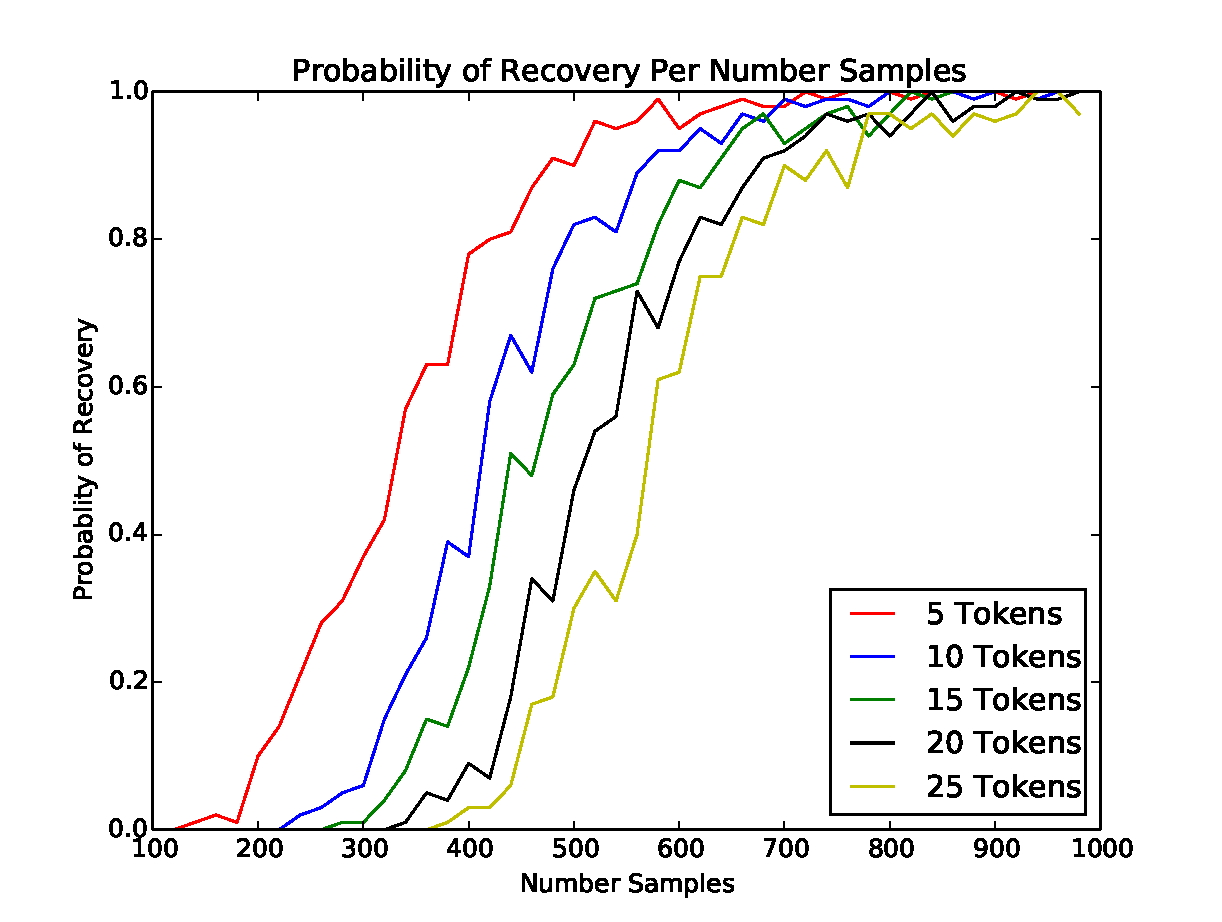
\includegraphics[width=3.5in]{./recovery_probability_per_samples.pdf}
	\caption{Recovery Probability}
	\label{fig:recovery_probability}
\end{figure}

